\documentclass[a4paper, reqno, 12pt, openbib]{article} % document class amsart class, draft points out the lines that are two long, reqno puts equations numbers to the right
\usepackage{geometry}\geometry{a4paper,total={170mm,250mm},left=20mm,top=25mm} % define margins of the document
\usepackage{graphicx} % package to load illustrations
\usepackage{listings} % package to read a programming language if included
\usepackage{float} % package needed to fix figures in place
\newtheorem{theorem}{Theorem}[section] % to input theorems
\newtheorem{corollary}{Corollary}[theorem] % to input collary
\newtheorem{lemma}[theorem]{Lemma} % to input lemmas
\usepackage[utf8]{inputenc}
\usepackage[english]{babel}
\usepackage{amssymb}
\usepackage{amsmath}
\usepackage{color} 
\usepackage{hyperref} % enable hyperlinks in the document 
\hypersetup{
    colorlinks = true,
    linktoc = all,
    citecolor=green,
    filecolor=black,
    linkcolor=blue,
    urlcolor=red
}
% --------------------------- PREAMBLE --------------------------------------------%
\begin{document}
\title{Filtering and Identification notes}
\author{Pradeep Janakiraman \thanks{TU Delft student from 2019-2021, notes written in Quarter 2 of AY 2020-2021}\\
3ME department\\
TU Delft, The Netherlands\\
pradeepjanakiraman@student.tudelft.nl}
\date{9 November 2020}
\maketitle
%---------------------------- TITLE PAGE ------------------------------------------%
\newpage
\tableofcontents
\newpage
%-----------
\section{Motivation behind the course}
\subsection{Identifying linear static models}
The first part of the course will involve trying find the parameters of a function $f(\theta)$ that will be used to model a real system with measurements $y$. The course will focus on linear models however, so $f(\theta) = F\theta$. The problem is then reduced to: 
\begin{equation}
	\min_{\theta} \|y - F\theta\|^{2}
\end{equation}
\subsection{Filtering} 
In the second part of the course, instead of identifying static parameters of a model, we will be identifying states of a system that vary with time. In this scenario, we are aware of the models that define the system and we want to make a prediction of the next state. We are also given the current state and current output, and have access to the history of states and outputs. The problem can be written as: 
\begin{align}
	x_{k+1} &= Ax_{k} + Bu_{k}\\
	y_{k} &= Cx_{k} + Du_{k}
\end{align} 
\subsection{Identification} 
In the last part of the course, we face the situation where we do not have any knowledge of the model that defines the system. We are then tasked to find the $(A, B, C, D)$ matrices or parametric models in the form of $f(\theta)$. 


\section{Lecture 1 - Electrostatics}
We first define an electric field $\vec{E}$ as the electrical force on a unit charge at position $2$ due to a to a point charge $q$ at position $1$. From coloumb's law, we can then write: 
\begin{equation}
	\label{formula for electric field}
	\vec{E} = \frac{1}{4\pi \epsilon_{0}} \frac{q}{r^{2}} \vec{e}_{12}
\end{equation}
$\vec{e}_{12}$ is the unit vector in the direction of the straight line between position 1 and 2. It should be stressed that $E$ is a vector and as 3 components along the 3 coordinate axes. Placing a unit charge anywhere in the electric field would result in a force on the unit charge given by \autoref{formula for electric field}. We then consider the work done on a unit charge to move it from an initial position to another postion. We know that, 
\begin{equation}
	W = -\int_{b}^{a} \vec{F} \cdot d\vec{s}
\end{equation}
Since we are only considering unit charges however, this can be re-written as: 
\begin{equation}
	\label{work equation}
	W = -\int_{b}^{a} \vec{E} \cdot d\vec{s}
\end{equation}
The above equation is really 3 integral formulas, one for each component. Now we note that the vector field $\vec{E}$ has some properties. 
\begin{itemize}
	\item The vector field is symmetric about the source point charge. 
	\item The vector field points in the radial direction with the source point charge at the center
\end{itemize}
So although the integal in \autoref{work equation} leads to different results depending on the path from $a$ to $b$, because of these two properties the integral becomes independent of the path and only depends on the positions of $a$ and $b$. Because of this we can write the result of the integral as follows: 
\begin{equation}
	-\int_{b}^{a} \vec{E} \cdot d\vec{s} = \phi(b) - \phi(a)
\end{equation}
$\phi(a, b)$ is the electric potential at points $a$ and $b$. From the figure below, we can see why this would be true. If we force the path we take from $a$ to $b$ to pass through $P_{0}$ we would get the result above. Usually $P_{0}$ is taken at $\infty$. 
\begin{figure}[H]
	\centering 
	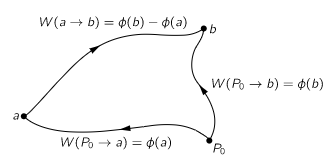
\includegraphics[scale = 0.5]{Lecture 1/images/path independence}
	\caption{A path moving from $a$ to $b$ is made to pass through $P_{0}$, which is usually taken at $\infty$ with 0 potential}
	\label{Illustration of the result obtained earlier}
\end{figure}
Then we can write: 
\begin{align}
	\phi(a) &= -\int_{\infty}^{a} \vec{E} \cdot d\vec{s}\\
	&= \frac{1}{4\pi \epsilon_{0}} \frac{q}{r_{a}} 
\end{align}
It should be noted that the above holds true only when the source point charge is at the origin. If the source is not at the origin, then the new distance must be taken instead of $r_{a}$. The principle of superpostion cen then be invoked for the case when there is more than once source point charge and we can write: 
\begin{align}
	\phi(1) &= \sum_{i} \frac{1}{4\pi \epsilon_{0}}\frac{q_{i}}{r_{1i}}\\
	&= \frac{1}{4\pi \epsilon_{0}}\int_{V(2)}\frac{\rho(2) dV_{2}}{r_{12}}
\end{align}
The second equation above uses the concept of a charge density $\rho$ that characterises many charges over a certain, summing up the charge density multiplied with elemental volumes would result in the total charge at the $r_{12}$. We can now go back to the result where the integral in \autoref{work equation} is path independent. We have already arrived at such a result previously in \autoref{line integral def}. It implies the following: 
\begin{align}
	-\int_{b}^{a} \vec{E} \cdot d\vec{s} &= \phi(b) - \phi(a)\\
	\int_{b}^{a} -\vec{\nabla}\phi \cdot d\vec{s} &= \phi(b) - \phi(a)\\
	\vec{E} &= -\vec{\nabla}\phi
\end{align}
However, we have already gone through the properties of double derivatives in \autoref{curl grad} and using that relationship, we can define: 
\begin{equation}
	\label{Maxwell eqn 2 for statics}
	\vec{\nabla} \times \vec{E} = 0
\end{equation}
Which is one Maxwell's equations for electrostatics. 
	




















\end{document}